%================ch1======================================
\chapter{Graphs and Their Applications}\label{ch1}
\section{Exercises}
    \begin{enumerate}[leftmargin=1.5em]
      \item {
        Study your campus map and model the road network inside your campus by a graph.
        
        \begin{description}[leftmargin=0em]
           \item[Answer:] {
                {[}Do it yourself{]}
            }
        \end{description}
      }
      \item {
        Construct a graph to represent the adjacency relationship of rooms in a floor of your university building.
        
        \begin{description}[leftmargin=0em]
           \item[Answer:] {
                {[}Do it yourself{]}\\
                Some examples taken from a floor plan paper \cite{floor_plan} in Figure \ref{fig:1_2_floorplan_to_graph}
                \begin{figure}[ht]
                    \centering
                    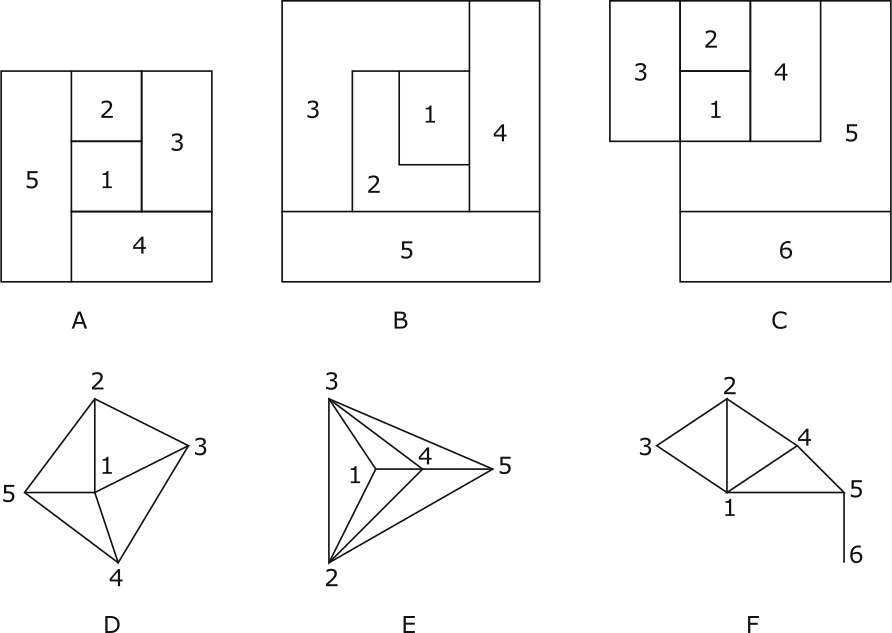
\includegraphics[width = 0.8\textwidth]{1_2_floorplan_to_graph.pdf}
                    \caption{Floor plan}
                    \label{fig:1_2_floorplan_to_graph}
                \end{figure}.
            }
        \end{description}
      }
      \item {
        Consider a party where there are exactly two alternate options of foods for each category of foods as follows. Rice: plane/yellow, Curry: fish/chicken, Naan: plain/butter, Kebab: chicken/mutton, Fruit: banana/mango, Drink: tea/coffee. Registered participants of the party gave their options as in Figure \ref{fig:1_3_table_food_opt}. Two participants conflict in their options if they give different options in the same category. Represent the conflicts of the participants using a conflict graph where each participant is represented by a vertex and there is an edge between two vertices if the corresponding participants conflict. By observing the conflict graph, find out the minimum number of persons whose absence divides the participants into two conflict free groups.
        \begin{figure}[H]
            \centering
            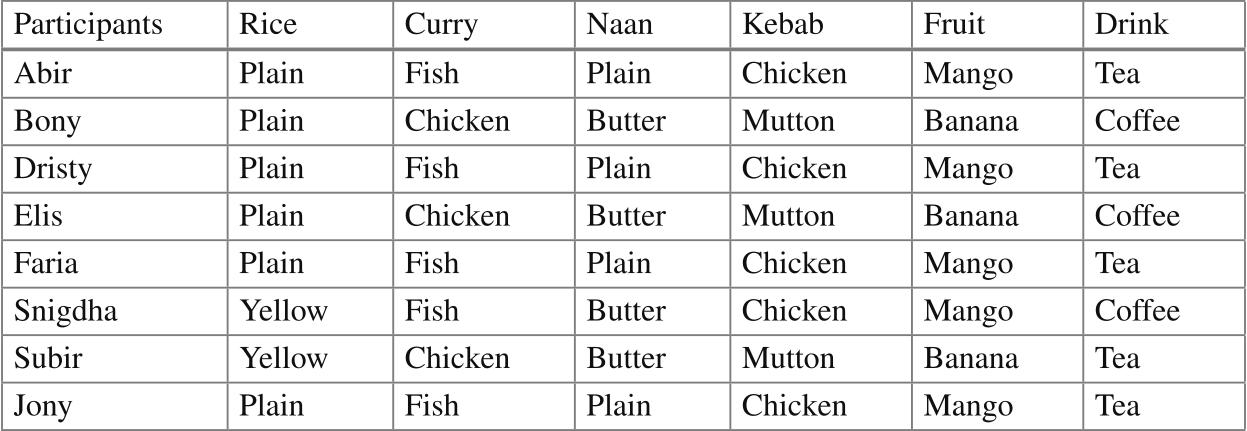
\includegraphics[width = 1\textwidth]{1_3_table_food_opt.pdf}
            \caption{Food option}
            \label{fig:1_3_table_food_opt}
        \end{figure}
        
        \begin{description}[leftmargin=0em]
           \item[Answer:] {
                Conflict graph Figure \ref{fig:1_3_conflict_graph}
                \begin{figure}[H]
                    \centering
                    \includegraphics[width = 0.8\textwidth]{1_3_conflict_graph.pdf}
                    \caption{Conflict graph}
                    \label{fig:1_3_conflict_graph}
                \end{figure}
                
                Conflict free groups: \{Abir, Dristy, Faria, Jony\}, \{Bony, Elis\}, \{Subir\}, \{Snigdha\}.\\
                Exclude 2 persons namely Subir and Snigdha to get two conflict free groups \{Abir, Dristy, Faria, Jony\} and \{Bony, Elis\}
            }
        \end{description}
      }
      \item {
        There are five jobs $\{J_1, J_2, J_3, J_4, J_5\}$ in a company for which there are five workers $A, B, C, D$ and $E$ to do those jobs. However, everybody does not have expertise to do every job. Their expertise is as follows: $A = \{J_1, J_2, J_3\}$, $B = \{J_2, J_4\}$, $C = \{J_1, J_3, J_5\}$, $D = \{J_3, J_5\}$, $E = \{J_1, J_5\}$. Develop a graph model to represent the job expertise of the persons and find an assignment of jobs to the workers such that every worker can do a job.
        
        \begin{description}[leftmargin=0em]
           \item[Answer:] {
                Job assignment graph Figure \ref{fig:1_4_job_assg}
                \begin{figure}[H]
                    \centering
                    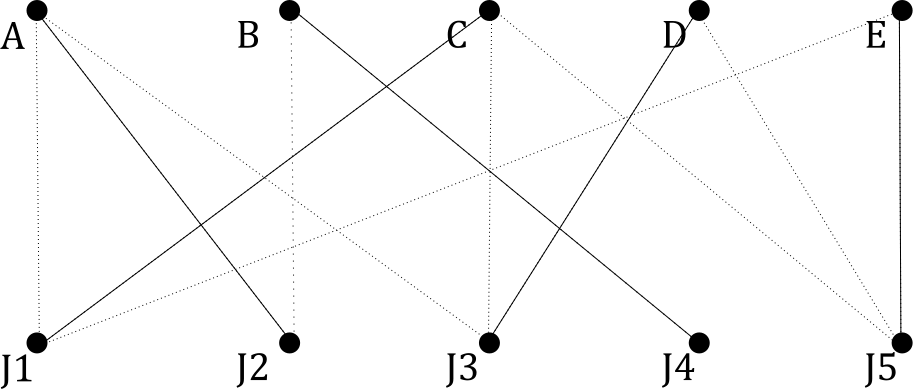
\includegraphics[width = 0.8\textwidth]{1_4_job_assg.pdf}
                    \caption{Job assignment graph}
                    \label{fig:1_4_job_assg}
                \end{figure}
            }
        \end{description}
      }
      \item {
        An industry has 600 square meter rectangular area on a floor of a building where it needs to establish four processing units $A, B, C$, and $D$. Processing units $A$ and $D$ require 100 square meter area each whereas $B$ and $C$ require 200 square meter each. Furthermore, the following adjacency requirements must be satisfied: $B, C$, and $D$ should be adjacent to $A; A$ and $D$ should be adjacent to $B; A$ and $D$ should be adjacent to $C;$ and $A, B$, and $C$ should be adjacent to $D$. Can you construct a floor layout where the space for each processing unit will be a rectangle? Propose a suitable layout in your justification.
        
        \begin{description}[leftmargin=0em]
           \item[Answer:] {
                Industry unit layout Figure \ref{fig:1_5_floor_plan}
                \begin{figure}[H]
                    \centering
                    \includegraphics[width = 0.8\textwidth]{1_5_floor_plan.pdf}
                    \caption{Industry unit layout}
                    \label{fig:1_5_floor_plan}
                \end{figure}
            }
        \end{description}
      }
    \end{enumerate}
    
% \section{Solutions}
%     \begin{enumerate}[leftmargin=1.5em]
%       \item {
%         % Study your campus map and model the road network inside your campus by a graph.
        
%         \begin{description}[leftmargin=0em]
%           \item[Answer:] {
%                 {[}Do it yourself{]}
%             }
%         \end{description}
%       }
%       \item {
%         % Construct a graph to represent the adjacency relationship of rooms in a floor of your university building.
        
%         \begin{description}[leftmargin=0em]
%           \item[Answer:] {
%                 {[}Do it yourself{]}\\
%                 Some examples taken from a floor plan paper \cite{floor_plan} in Figure \ref{fig:1_2_floorplan_to_graph}
%                 \begin{figure}[ht]
%                     \centering
%                     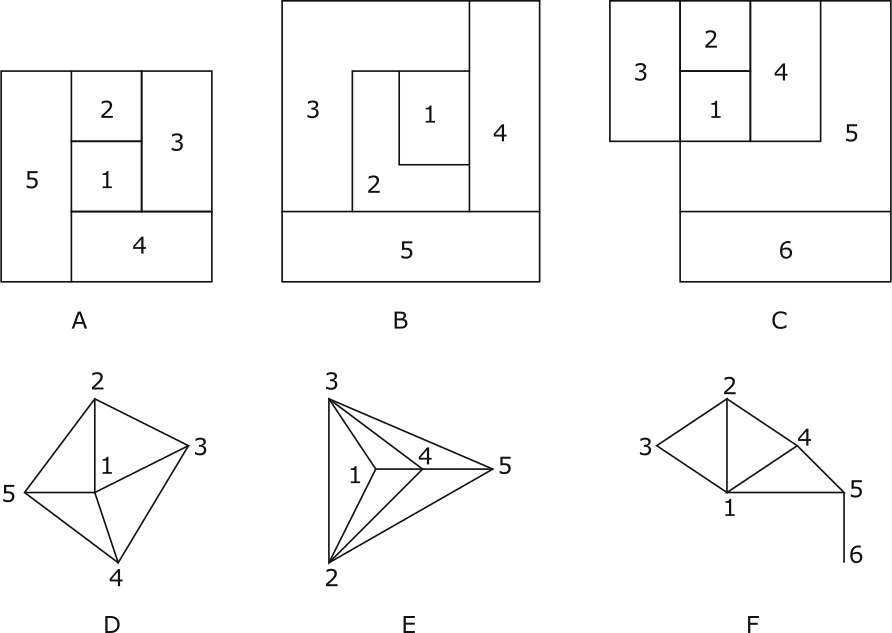
\includegraphics[width = 0.8\textwidth]{1_2_floorplan_to_graph.pdf}
%                     \caption{Floor plan}
%                     \label{fig:1_2_floorplan_to_graph}
%                 \end{figure}.
%             }
%         \end{description}
%       }
%       \item {
%         % Consider a party where there are exactly two alternate options of foods for each category of foods as follows. Rice: plane/yellow, Curry: fish/chicken, Naan: plain/butter, Kebab: chicken/mutton, Fruit: banana/mango, Drink: tea/coffee. Registered participants of the party gave their options as in Figure \ref{fig:1_3_table_food_opt}. Two participants conflict in their options if they give different options in the same category. Represent the conflicts of the participants using a conflict graph where each participant is represented by a vertex and there is an edge between two vertices if the corresponding participants conflict. By observing the conflict graph, find out the minimum number of persons whose absence divides the participants into two conflict free groups.
%         % \begin{figure}[H]
%         %     \centering
%         %     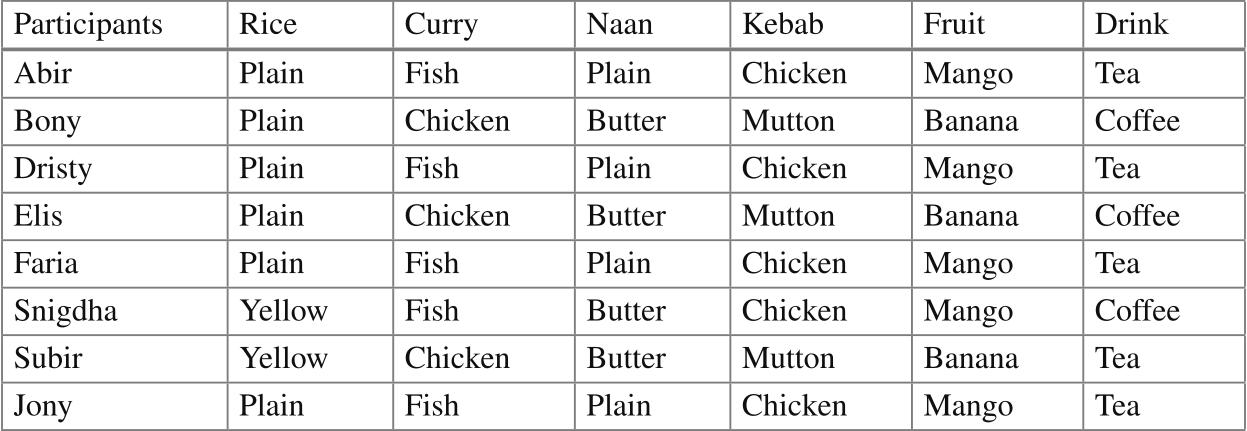
\includegraphics[width = 1\textwidth]{1_3_table_food_opt.pdf}
%         %     \caption{Food option}
%         %     \label{fig:1_3_table_food_opt}
%         % \end{figure}
        
%         \begin{description}[leftmargin=0em]
%           \item[Answer:] {
%                 Conflict graph Figure \ref{fig:1_3_conflict_graph}
%                 \begin{figure}[H]
%                     \centering
%                     \includegraphics[width = 0.8\textwidth]{1_3_conflict_graph.pdf}
%                     \caption{Conflict graph}
%                     \label{fig:1_3_conflict_graph}
%                 \end{figure}
                
%                 Conflict free groups: \{Abir, Dristy, Faria, Jony\}, \{Bony, Elis\}, \{Subir\}, \{Snigdha\}.\\
%                 Exclude 2 persons namely Subir and Snigdha to get two conflict free groups \{Abir, Dristy, Faria, Jony\} and \{Bony, Elis\}
%             }
%         \end{description}
%       }
%       \item {
%         % There are five jobs $\{J_1, J_2, J_3, J_4, J_5\}$ in a company for which there are five workers $A, B, C, D$ and $E$ to do those jobs. However, everybody does not have expertise to do every job. Their expertise is as follows: $A = \{J_1, J_2, J_3\}$, $B = \{J_2, J_4\}$, $C = \{J_1, J_3, J_5\}$, $D = \{J_3, J_5\}$, $E = \{J_1, J_5\}$. Develop a graph model to represent the job expertise of the persons and find an assignment of jobs to the workers such that every worker can do a job.
        
%         \begin{description}[leftmargin=0em]
%           \item[Answer:] {
%                 Job assignment graph Figure \ref{fig:1_4_job_assg}
%                 \begin{figure}[H]
%                     \centering
%                     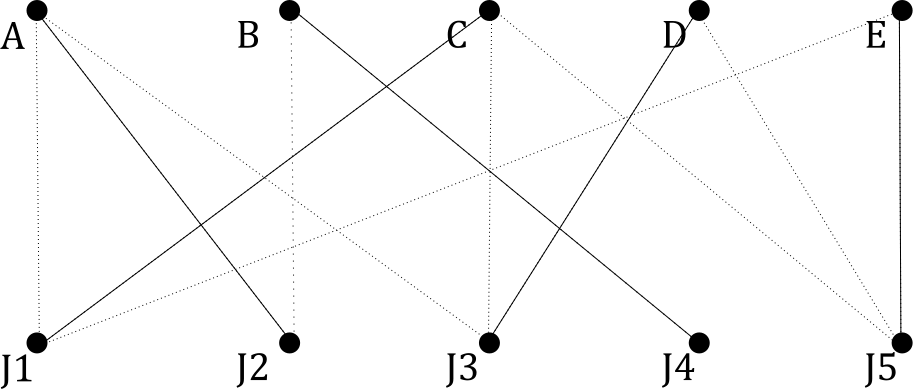
\includegraphics[width = 0.8\textwidth]{1_4_job_assg.pdf}
%                     \caption{Job assignment graph}
%                     \label{fig:1_4_job_assg}
%                 \end{figure}
%             }
%         \end{description}
%       }
%       \item {
%         % An industry has 600 square meter rectangular area on a floor of a building where it needs to establish four processing units $A, B, C$, and $D$. Processing units $A$ and $D$ require 100 square meter area each whereas $B$ and $C$ require 200 square meter each. Furthermore, the following adjacency requirements must be satisfied: $B, C$, and $D$ should be adjacent to $A; A$ and $D$ should be adjacent to $B; A$ and $D$ should be adjacent to $C;$ and $A, B$, and $C$ should be adjacent to $D$. Can you construct a floor layout where the space for each processing unit will be a rectangle? Propose a suitable layout in your justification.
        
%         \begin{description}[leftmargin=0em]
%           \item[Answer:] {
%                 Industry unit layout Figure \ref{fig:1_5_floor_plan}
%                 \begin{figure}[H]
%                     \centering
%                     \includegraphics[width = 0.8\textwidth]{1_5_floor_plan.pdf}
%                     \caption{Industry unit layout}
%                     \label{fig:1_5_floor_plan}
%                 \end{figure}
%             }
%         \end{description}
%       }
%     \end{enumerate}
